\section{VL 02: Welchen nutzen stiftet IT in Organisationen?}
Thema: Wofür werden Informationssysteme in Unternehmen eingesetzt und was bewirkt das?

Informationssysteme
\begin{itemize}
	\item Informieren
	\item Erleichtern die Kommunikation
	\item Koordinieren
	\item Automatisieren
\end{itemize}

Wichtige Definitionen:
\begin{description}
	\item[Unternehmung] Ein \em Betrieb \em in einem marktwirtschaftlichen System.
	\item[Betrieb] Eine planvoll organisierte Wirtschaftseinheit, in der Produktionsfaktoren kombiniert werden, um Güter und Dienstleistungen herzustellen und abzusetzen.
	\item[Informationssystem] Soziotechnische (Mensch \em und \em Maschine) Systeme, die der optimalen Bereitstellung von Information und Kommunikation nach wirtschaftlichen Kriterien dienen.
\end{description}

Organisation mit Informationssystem:
\begin{center}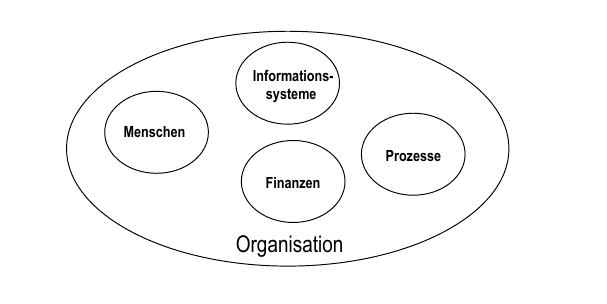
\includegraphics[width=0.8\textwidth]{IS-Kontext.png}\end{center}

In vielen Diagrammen und Studien kann man sehen: IT wirkt stark zeitversetzt und (fast nur) in Verbindung mit einer Dezentralisierung der Organisationsstruktur.

Der Nutzen von Informationssystemen in Unternehmungen wird durch folgendes Diagramm zusammengefasst:

\begin{center}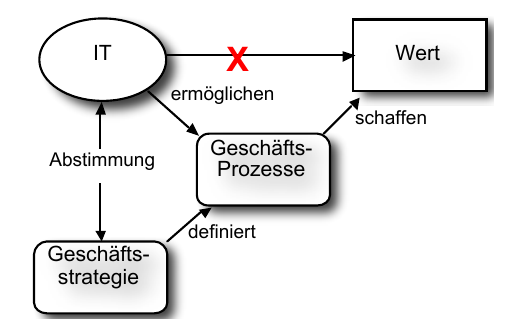
\includegraphics[width=0.9\textwidth]{IS-Nutzen.png}\end{center}

Die Beispiel-Klausuraufgabe war, dieses Diagramm zu beschriften.